\chapter{About split, interval and permutation graphs}
\label{sec:23}

\abstract*{ The last chapter of this book eventually presents some famous classes of perfect graphs, namely comparability, interval, permutation and split graphs. We first generate a random graph instance which models at the same time an interval, a comparability, a split and a permutation graph. The importance to be an interval is illustrated with \Berge 's mystery story. We discuss furthermore the generation of permutation graphs and close with how to recognize that a given graph is in fact a permutation graph.}

\abstract{ The last chapter of this book eventually presents some famous classes of perfect graphs, namely comparability, interval, permutation and split graphs. We first present an example of a graph which is at the same time a triangulated, a comparability, a split and a permutation graph. The importance to be an interval is illustrated with \Berge 's mystery story. We discuss furthermore the generation of permutation graphs and close with how to recognize that a given graph is in fact a permutation graph.}

\section{A 'multiply' perfect graph}
\label{sec:23.1}

A graph \texttt{g} is called:
\begin{itemize}
\item \Berge or \emph{perfect} when \texttt{g} and its dual \texttt{-g} both don't contain any chordless odd cycles of length greater than $3$ \citep*{BER-1963,CHU-2006}\index{BergeGraph@\Berge graph}; 
\item \emph{Triangulated} graph when \texttt{g} does not contain any \emph{chordless cycle} of length 4 and more;\index{triangulated graph}
\end{itemize}

\begin{definition}[Some perfect graph classes]
\noindent Following Martin Golumbic (see \citet[p. 149]{GOL-2004}), we call a given graph \texttt{g}:
\begin{itemize}
\item \emph{Comparability} graph when \texttt{g}  is \emph{transitively orientable};\index{comparability graph}
\item \emph{Interval} graph when \texttt{g} is \emph{triangulated} and its dual \texttt{-g} is a \emph{comparability} graph;\index{comparability graph}
\item \emph{Permutation} graph when \texttt{g} and its dual \texttt{-g} both are \emph{comparability} graphs;\index{permutation graph}
\item \emph{Split} graph when \texttt{g} and its dual \texttt{-g} bothare \emph{triangulated} graphs.\index{split graph}
\end{itemize}
\end{definition}

To illustrate these \emph{perfect} graph classes, we will generate from $8$ intervals, randomly chosen in the default integer range $[0,10]$, a \texttt{RandomIntervalInter\-sectionsGraph} instance \texttt{g} (see Line 2 below).\index{RandomIntervalIntersectionsGraph@\texttt{RandomIntervalIntersectionsGraph} class} 
\begin{lstlisting}
>>> from graphs import\
...             RandomIntervalIntersectionsGraph
>>> g = RandomIntervalIntersectionsGraph(\
...                          order=8,seed=100)
>>> g
  *------- Graph instance description ------*
   Instance class   : RandomIntervalIntersectionsGraph
   Instance name    : randIntervalIntersections
   Seed             : 100
   Graph Order      : 8
   Graph Size       : 23
   Valuation domain : [-1.0; 1.0]
   Attributes       : ['seed', 'name', 'order',
        'intervals', 'vertices', 'valuationDomain',
        'edges', 'size', 'gamma']
>>> print(g.intervals)
  [(2,7), (2,7), (5,6), (6,8), (1,8), (1,1), (4,7), (0,10)]
\end{lstlisting}

With \texttt{seed = 100}, we obtain here an \emph{interval graph}, in fact a \emph{perfect graph}, which is \emph{conjointly} a \emph{triangulated}, a \emph{comparability}, a \emph{split} and a \emph{permutation} graph (see Listing~\vref{list:23.1} Lines 6, 10, 14 and Fig.~\vref{fig:23.1}).\index{isPerfectGraph@\texttt{isPerfectGraph()}}\index{isSpliGraph@\texttt{isSplitGraph()}}\index{isIntervalGraph@\texttt{isIntervalGraph()}}\index{isPermutationGraph@\texttt{isPermutationGraph()}}
\begin{lstlisting}[caption={Testing perfect graph categories.},label=list:23.1,basicstyle=\ttfamily\scriptsize]
>>> g.isPerfectGraph(Comments=True)
  Graph randIntervalIntersections is perfect !
>>> g.isIntervalGraph(Comments=True)
  Graph 'randIntervalIntersections' is triangulated.
  Graph 'dual_randIntervalIntersections' is transitively orientable.
  => Graph 'randIntervalIntersections' is an interval graph.
>>> g.isSplitGraph(Comments=True)
  Graph 'randIntervalIntersections' is triangulated.
  Graph 'dual_randIntervalIntersections' is triangulated.
  => Graph 'randIntervalIntersections' is a split graph.
>>> g.isPermutationGraph(Comments=True)
  Graph 'randIntervalIntersections' is transitively orientable.
  Graph 'dual_randIntervalIntersections' is transitively orientable.
  => Graph 'randIntervalIntersections' is a permutation graph.
>>> print(g.computePermutation())
  ['v5', 'v6', 'v4', 'v2', 'v1', 'v3', 'v7', 'v8']
  ['v8', 'v6', 'v1', 'v2', 'v3', 'v4', 'v7', 'v5']
  [8, 2, 6, 5, 7, 4, 3, 1]
>>> g.exportGraphViz('randomSplitGraph')
  *---- exporting a dot file for GraphViz tools ---------*
   Exporting to randomSplitGraph.dot
   fdp -Tpng randomSplitGraph.dot -o randomSplitGraph.png
\end{lstlisting}
\begin{figure}[h]
\sidecaption[t]
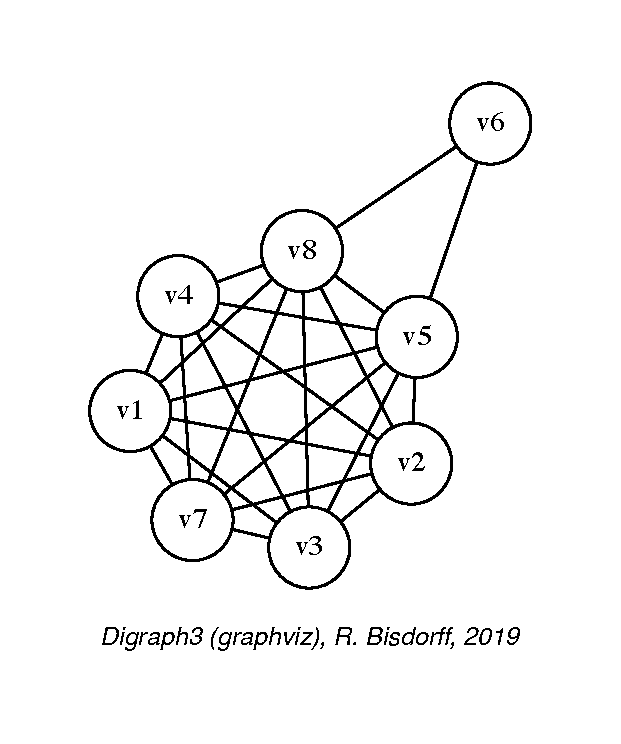
\includegraphics[width=7cm]{Figures/23-1-randomSplitGraph.pdf}
\caption{A conjointly triangulated, comparability, interval, permutation and split graph. In the Figure here one may readily recognize the essential characteristic of split graphs, namely being always splitable into two disjoint sub-graphs: an \emph{independent choice} \{\texttt{v6}\} and a \emph{clique}  --\{\texttt{v1}, \texttt{v2}, \texttt{v3}, \texttt{v4}, \texttt{v5}, \texttt{v7}, \texttt{v8}\}-- which explains their name} 
\label{fig:23.1}       % Give a unique label
\end{figure}
Notice however that the four properties:
\begin{enumerate}[nosep]
\item $g$ is a \emph{comparability} graph;
\item $g$ is a \emph{co-comparability} graph, i.e. $-g$ is a comparability graph;
\item $g$ is a \emph{triangulated} graph;
\item $g$ is a \emph{co-triangulated} graph, i.e. $-g$ is a comparability graph;
\end{enumerate}
are independent of one another (see \citet[p. 275]{GOL-2004}).

\section{Who is the liar?}
\label{sec:23.2}

Claude \Berge's famous mystery story related by \citet[p. 20]{GOL-2004} may well illustrate the importance of being an \emph{interval} graph.

Suppose the file \texttt{berge.py} \footnote{The file \texttt{berge.py} is provided in the \texttt{examples} directory of the \Digraph resources.} contains the following \texttt{Graph} instance data:
\begin{lstlisting}
  vertices = {
    'A': {'name': 'Abe', 'shortName': 'A'},
    'B': {'name': 'Burt', 'shortName': 'B'},
    'C': {'name': 'Charlotte', 'shortName': 'C'},
    'D': {'name': 'Desmond', 'shortName': 'D'},
    'E': {'name': 'Eddie', 'shortName': 'E'},
    'I': {'name': 'Ida', 'shortName': 'I'},
    }
  valuationDomain = {'min':-1,'med':0,'max':1}
  edges = {
    frozenset(['A','B']) : 1, 
    frozenset(['A','C']) : -1, 
    frozenset(['A','D']) : 1, 
    frozenset(['A','E']) : 1, 
    frozenset(['A','I']) : -1, 
    frozenset(['B','C']) : -1, 
    frozenset(['B','D']) : -1, 
    frozenset(['B','E']) : 1, 
    frozenset(['B','I']) : 1, 
    frozenset(['C','D']) : 1, 
    frozenset(['C','E']) : 1, 
    frozenset(['C','I']) : 1, 
    frozenset(['D','E']) : -1, 
    frozenset(['D','I']) : 1, 
    frozenset(['E','I']) : 1, 
    }
\end{lstlisting}

Six professors (labeled \texttt{A}, \texttt{B}, \texttt{C}, \texttt{D}, \texttt{E} and \texttt{I}) had been to the library on the day that a rare tractate was stolen. Each entered once, stayed for some time, and then left. If two professors were in the library at the same time, then at least one of them saw the other. Detectives questioned the professors and gathered the testimonies that \emph{Abe} saw \emph{Burt} and \emph{Eddie}; \emph{Burt} saw \emph{Abe} and \emph{Ida}; \emph{Charlotte} saw \emph{Desmond} and \emph{Ida}; \emph{Desmond} saw \emph{Abe} and \emph{Ida}; \emph{Eddie} saw \emph{Burt} and \emph{Ida}; and \emph{Ida} saw \emph{Charlotte} and \emph{Eddie}. This data is gathered in the previous file, where each positive edge $\{x,y\}$ models the testimony that, either $x$ saw $y$, or $y$ saw $x$.
\begin{lstlisting}
>>> from graphs import Graph
>>> g = Graph('berge')
>>> g.showShort()
  *---- short description of the graph ----*
   Name             : 'berge'
   Vertices         :  ['A', 'B', 'C', 'D', 'E', 'I']
   Valuation domain :  {'min': -1, 'med': 0, 'max': 1}
   Gamma function   : 
    A -> ['D', 'B', 'E']
    B -> ['E', 'I', 'A']
    C -> ['E', 'D', 'I']
    D -> ['C', 'I', 'A']
    E -> ['C', 'B', 'I', 'A']
    I -> ['C', 'E', 'B', 'D']
>>> g.exportGraphViz('berge1')
  *---- exporting a dot file for GraphViz tools ---------*
   Exporting to berge1.dot
   fdp -Tpng berge1.dot -o berge1.png
\end{lstlisting}
\begin{figure}[h]
\sidecaption[t]
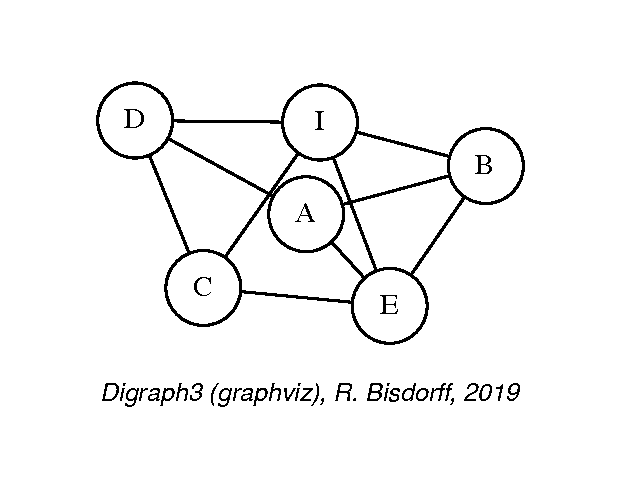
\includegraphics[width=7cm]{Figures/23-2-berge1.pdf}
\caption{Graph representation of the testimonies of the professors} 
\label{fig:23.2}       % Give a unique label
\end{figure}

From graph theory we know that time interval intersections graphs must in fact be interval graph instances, i.e. \emph{triangulated} and \emph{co-comparative} graphs. The testimonies graph shown in Fig.~\vref{fig:23.2} should therefore not contain any chordless cycle of four and more vertices. Now, the presence or not of such chordless cycles in the testimonies graph may be checked with the \texttt{computeChordlessCycles()} method \citep{BIS-2010}.\index{computeChordlessCycles@\emph{computeChordlessCycles()}}
\begin{lstlisting}
>>> g.computeChordlessCycles()
  Chordless cycle certificate: ['D','C','E','A','D']
  Chordless cycle certificate: ['D','I','E','A','D']
  Chordless cycle certificate: ['D','I','B','A','D']
  [(['D','C','E','A','D'],frozenset({'C','D','E','A'})),
  (['D','I','E','A','D'],frozenset({'D','E','I','A'})),
  (['D','I','B','A','D'],frozenset({'D','B','I','A'}))]
\end{lstlisting}
We see in the Listing above three intersection cycles of length 4, which is impossible to occur on the linear time line. Obviously one professor lied!

And it is \emph{Desmond}. If we doubt his testimony that he saw \emph{Abe} (see Line 1 below), we obtain indeed in Fig.~\vref{fig:23.3} a triangulated graph instance whose dual is a comparability graph.\index{setEdgeValue@\texttt{setEdgeValue()}}
\begin{lstlisting}
>>> g.setEdgeValue( ('D','A'), 0)
>>> g.showShort()
  *---- short description of the graph ----*
   Name             : 'berge'
   Vertices         :  ['A','B','C','D','E','I']
   Valuation domain :  {'med': 0,'min': -1,'max': 1}
   Gamma function   : 
    A -> ['B', 'E']
    B -> ['A', 'I', 'E']
    C -> ['I', 'E', 'D']
    D -> ['I', 'C']
    E -> ['A', 'I', 'B', 'C']
    I -> ['B', 'E', 'D', 'C']
>>> g.isIntervalGraph(Comments=True)
  Graph 'berge' is triangulated.
  Graph 'dual_berge' is transitively orientable.
  => Graph 'berge' is an interval graph.
>>> g.exportGraphViz('berge2')
  *---- exporting a dot file for GraphViz tools ---------*
   Exporting to berge2.dot
   fdp -Tpng berge2.dot -o berge2.png
\end{lstlisting}
\begin{figure}[h]
\sidecaption[t]
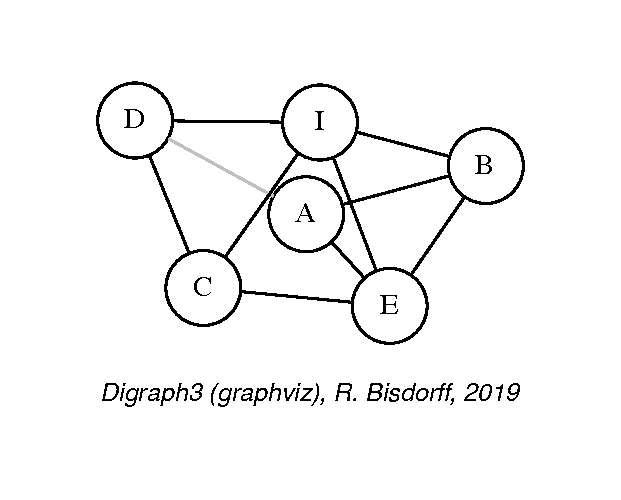
\includegraphics[width=7cm]{Figures/23-3-berge2.pdf}
\caption{The triangulated testimonies graph} 
\label{fig:23.3}       % Give a unique label
\end{figure}

\section{Generating permutation graphs}
\label{sec:23.3}

A graph is called a \emph{permutation} or \emph{inversion} graph if there exists a permutation of its list of vertices such that the graph is isomorphic to the inversions operated by the permutation in this list (see \citet[Chapter 7, pp 157-170]{GOL-2004}). This kind of graphs (see Fig.~\vref{fig:23.4} is also part of the class of perfect graphs.\index{PermutationGraph@\texttt{PermutationGraph} class}
\begin{lstlisting}
>>> from graphs import PermutationGraph
>>> g = PermutationGraph(permutation = [4,3,6,1,5,2])
>>> g
  *------- Graph instance description ------*
   Instance class   : PermutationGraph
   Instance name    : permutationGraph
   Graph Order      : 6
   Permutation      : [4, 3, 6, 1, 5, 2]
   Graph Size       : 9
   Valuation domain : [-1.00; 1.00]
   Attributes       : ['name', 'vertices', 'order',
                  'permutation', 'valuationDomain',
                  'edges', 'size', 'gamma']
>>> g.isPerfectGraph()
  True
>>> g.exportGraphViz(fileName='permutationGraph')
  *---- exporting a dot file for GraphViz tools ----*
   Exporting to permutationGraph.dot
   fdp -Tpng permutationGraph.dot\
                    -o permutationGraph.png
\end{lstlisting}
\begin{figure}[h]
\sidecaption[t]
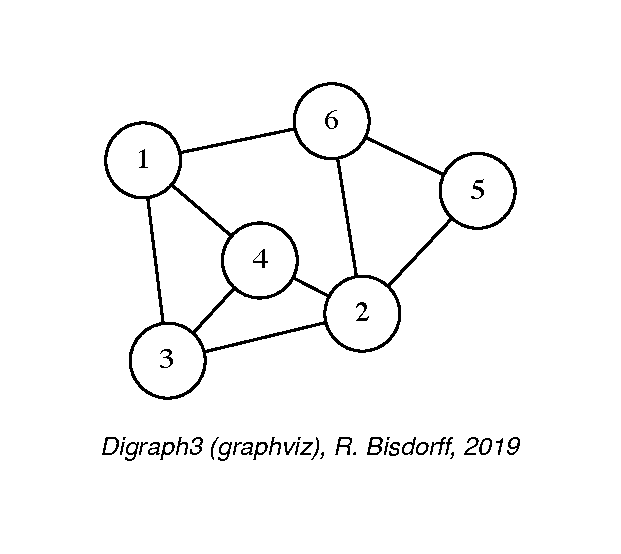
\includegraphics[width=7cm]{Figures/23-4-permutationGraph.pdf}
\caption{The default \Digraph permutation graph} 
\label{fig:23.4}       % Give a unique label
\end{figure}

By using color sorting queues, the minimal vertex coloring shown in Fig.~\vref{fig:23.5} is computable in $O\big(n log(n)\big)$ (see \citet{GOL-2004}).\index{computeMinimalVertexColoring@\texttt{computeMinimalVertexColoring()}}
\begin{lstlisting}
>>> g.computeMinimalVertexColoring(Comments=True)
    vertex 1: lightcoral
    vertex 2: lightcoral
    vertex 3: lightblue
    vertex 4: gold
    vertex 5: lightblue
    vertex 6: gold
>>> g.exportGraphViz(fileName='coloredPermutationGraph',\
...                  WithVertexColoring=True)
  *---- exporting a dot file for GraphViz tools -------*
   Exporting to coloredPermutationGraph.dot
   fdp -Tpng coloredPermutationGraph.dot\
       -o coloredPermutationGraph.png
\end{lstlisting}
\begin{figure}[h]
\sidecaption[t]
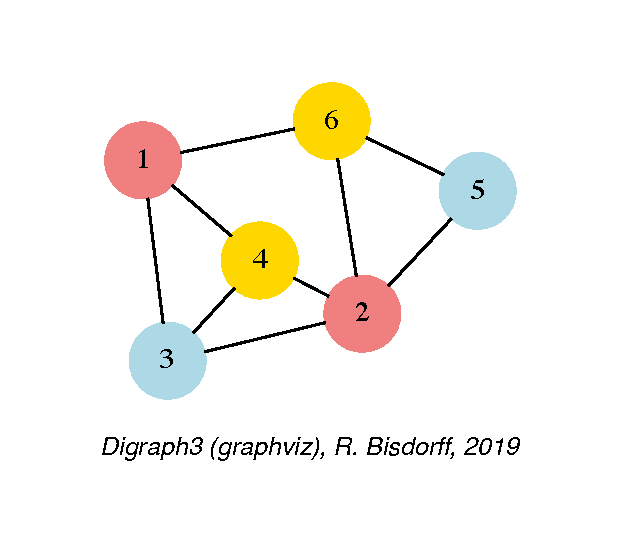
\includegraphics[width=6cm]{Figures/23-5-coloredPermutationGraph.pdf}
\caption{Minimal vertex coloring of the permutation graph.} 
\label{fig:23.5}       % Give a unique label
\end{figure}

The correspondingly colored \emph{matching diagram} of the nine inversions --the actual edges of the permutation graph--, which are induced by the given [4,3,6,1,5,2] permutation, may as well be drawn with the graphviz \texttt{neato} layout and explicitly positioned horizontal lists of vertices as shown in Fig.~\vref{fig:23.6}.\index{exportPermutationGraphViz@\texttt{exportPermutationGraphViz()}}
\begin{lstlisting}
>>> g.exportPermutationGraphViz(\
...                    WithEdgeColoring=True)
  *---- exporting a dot file for GraphViz tools ------*
   Exporting to perm_permutationGraph.dot
   neato -n -Tpng perm_permutationGraph.dot\
            -o perm_permutationGraph.png
\end{lstlisting}
\begin{figure}[h]
\sidecaption
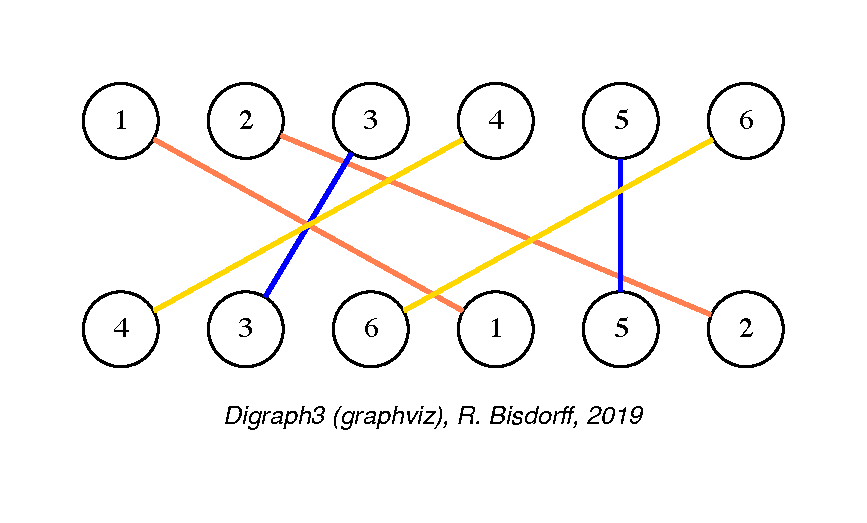
\includegraphics[width=10cm]{Figures/23-6-perm_permutationGraph.pdf}
\caption{Colored matching diagram of the permutation [4,3,6,1,5,2]} 
\label{fig:23.6}       % Give a unique label
\end{figure}

As mentioned before, a permutation graph and its dual are \emph{transitively orientable}. The \texttt{transitiveOrientation()} method\index{transitiveOrientation@\texttt{transitiveOrientation()}} constructs from a given permutation graph a digraph where each edge of the permutation graph is converted into an arc oriented in increasing alphabetic order of the adjacent vertices' keys (see \citet{GOL-2004}). This orientation of the edges of a permutation graph is always transitive and delivers a \emph{transitive ordering} of the vertices as shown in Fig.~\vref{fig:23.7}.\index{transitiveOrientation@\texttt{transitiveOrientation()}}
\begin{lstlisting}
>>> dg = g.transitiveOrientation()
>>> dg
  *------- Digraph instance description ------*
   Instance class   : TransitiveDigraph
   Instance name    : oriented_permutationGraph
   Digraph Order      : 6
   Digraph Size       : 9
   Valuation domain : [-1.00; 1.00]
   Determinateness  : 100.000
   Attributes       : ['name', 'order', 'actions',
                    'valuationdomain', 'relation',
                    'gamma', 'notGamma', 'size']
>>> print('Transitivity degree: %.3f' %\
...          dgd.computeTransitivityDegree() ) 
   Transitivity degree: 1.000
>>> dg.exportGraphViz(fileName='orientedPermGraph')
  *---- exporting a dot file for GraphViz tools -----*
   Exporting to orientedPermGraph.dot
   dot -Grankdir=TB -Tpng orientedPermGraph.dot\
                    -o orientedPermGraph.png
\end{lstlisting}
\begin{figure}[h]
\sidecaption[t]
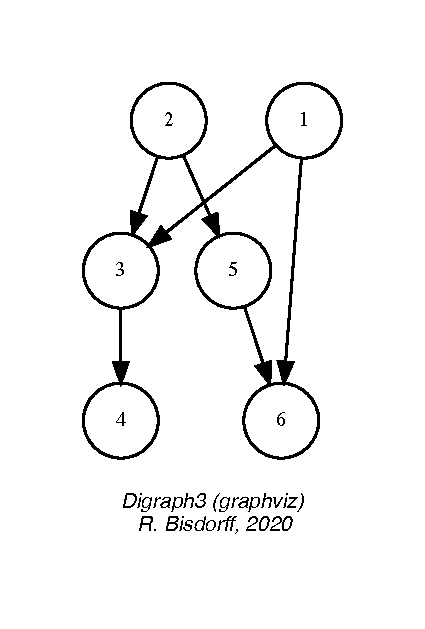
\includegraphics[width=5cm]{Figures/23-7-orientedPermGraph.pdf}
\caption{The transitive orientation of the permutation graph} 
\label{fig:23.7}       % Give a unique label
\end{figure}

The dual of a permutation graph is again a permutation graph and as such also transitively orientable.
\begin{lstlisting}
>>> dgd = (-g).transitiveOrientation()
>>> print('Dual transitivity degree: %.3f' %\
...            dgd.computeTransitivityDegree() )
   Dual transitivity degree: 1.00
\end{lstlisting}

\section{Recognizing permutation graphs}
\label{sec:23.4}

Now, a given graph \texttt{g} is a permutation graph if and only if both \texttt{g} \textbf{and} \texttt{-g} are transitively orientable. This  property gives a polynomial test procedure (in $O(n^3)$ due to the transitivity check) for recognizing permutation graphs.

Let us consider, for instance, the following random graph of order 8 generated with an edge probability of $40\%$ and a random seed equal to $4335$.
\begin{lstlisting}
>>> from graphs import RandomGraph
>>> g = RandomGraph(order=8,\
...                 edgeProbability=0.4,seed=4335)
>>> g
  *------- Graph instance description ------*
   Instance class   : RandomGraph
   Instance name    : randomGraph
   Seed             : 4335
   Edge probability : 0.4
   Graph Order      : 8
   Graph Size       : 10
   Valuation domain : [-1.00; 1.00]
   Attributes       : ['name', 'order', 'vertices',
                       'valuationDomain', 'seed',
                       'edges', 'size', 'gamma',
                       'edgeProbability']
>>> g.isPerfectGraph()
  True
>>> g.exportGraphViz(fileName='randomGraph4335')
  *---- exporting a dot file for GraphViz tools ----*
   Exporting to randomGraph4335.dot
   fdp -Tpdf randomGraph4335.dot -o randomGraph4335.pdf
\end{lstlisting}		    
\begin{figure}[h]
\sidecaption[t]
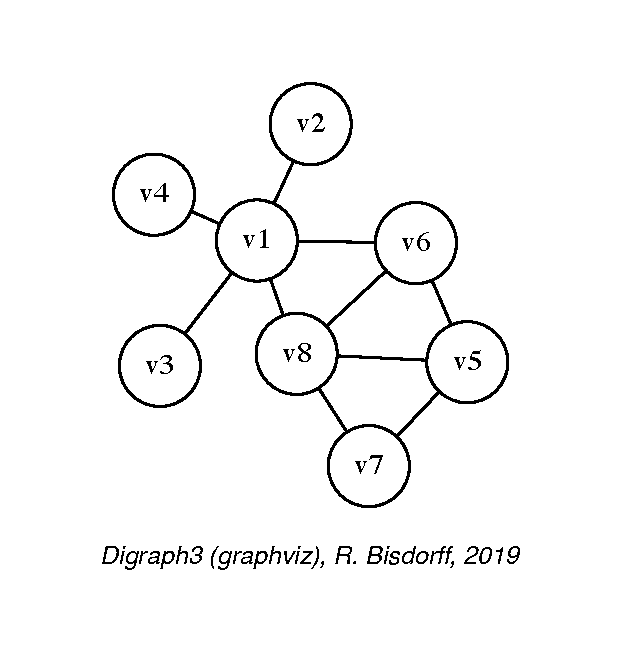
\includegraphics[width=6cm]{Figures/23-8-randomGraph4335.pdf}
\caption{Random graph of order 8 generated with edge probability $0.4$.} 
\label{fig:23.8}       % Give a unique label
\end{figure}

If the random perfect graph instance \texttt{g}, shown in Fig.~\vref{fig:23.8}, is indeed a permutation graph, \texttt{g} and its dual \texttt{-g} should be both \emph{transitively orientable}, i.e. comparability graphs (see \citet{GOL-2004}). With the \texttt{isComparabilityGraph()} test\index{isComparabilityGraph@\texttt{isComparabilityGraph()}}, we may easily check this fact. This method proceeds indeed by trying to construct a transitive neighbourhood decomposition of a given graph instance and, if successful, stores the resulting edge orientations into a \texttt{edgeOrientations} attribute (see \citet[p.129-132]{GOL-2004}).
\begin{lstlisting}[basicstyle=\scriptsize]
>>> if g.isComparabilityGraph():
...     print(g.edgeOrientations)  
 {('v1','v1'): 0, ('v1','v2'): 1, ('v2','v1'): -1, ('v1','v3'): 1,
  ('v3','v1'): -1, ('v1','v4'): 1, ('v4','v1'): -1, ('v1','v5'): 0,
  ('v5','v1'): 0, ('v1','v6'): 1, ('v6','v1'): -1, ('v1','v7'): 0,
  ('v7','v1'): 0, ('v1','v8'): 1, ('v8','v1'): -1, ('v2','v2'): 0,
  ('v2','v3'): 0, ('v3','v2'): 0, ('v2','v4'): 0, ('v4','v2'): 0,
  ('v2','v5'): 0, ('v5','v2'): 0, ('v2','v6'): 0, ('v6','v2'): 0,
  ('v2','v7'): 0, ('v7','v2'): 0, ('v2','v8'): 0, ('v8','v2'): 0,
  ('v3','v3'): 0, ('v3','v4'): 0, ('v4','v3'): 0, ('v3','v5'): 0,
  ('v5','v3'): 0, ('v3','v6'): 0, ('v6','v3'): 0, ('v3','v7'): 0,
  ('v7','v3'): 0, ('v3','v8'): 0, ('v8','v3'): 0, ('v4','v4'): 0,
  ('v4','v5'): 0, ('v5','v4'): 0, ('v4','v6'): 0, ('v6','v4'): 0,
  ('v4','v7'): 0, ('v7','v4'): 0, ('v4','v8'): 0, ('v8','v4'): 0,
  ('v5','v5'): 0, ('v5','v6'): 1, ('v6','v5'): -1, ('v5','v7'): 1,
  ('v7','v5'): -1, ('v5','v8'): 1, ('v8','v5'): -1, ('v6','v6'): 0,
  ('v6','v7'): 0, ('v7','v6'): 0, ('v6','v8'): 1, ('v8','v6'): -1,
  ('v7','v7'): 0, ('v7','v8'): 1, ('v8','v7'): -1, ('v8','v8'): 0}
>>> g.exportEdgeOrientationsGraphViz('transOrientGraph')
   *---- exporting a dot file for GraphViz tools ---------*
    Exporting to transOrientGraph.dot
    fdp -Tpng transOrientGraph.dot \
             -o transOrientGraph.png
\end{lstlisting}		    
\begin{figure}[h]
\sidecaption[t]
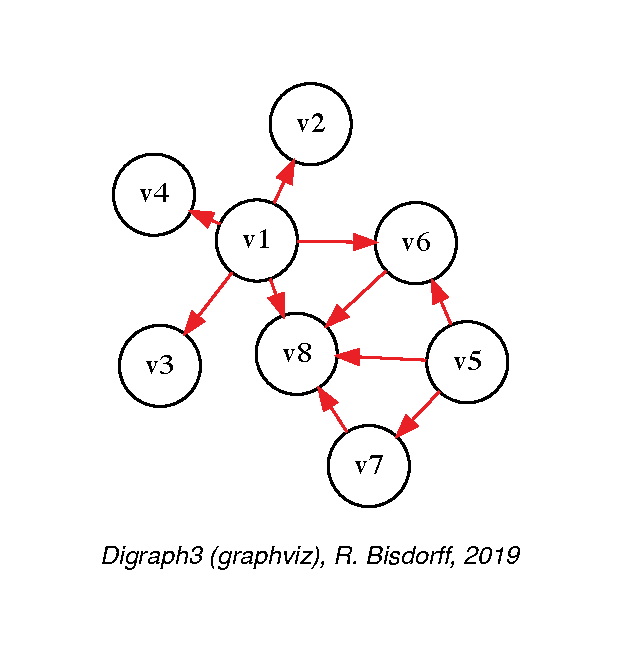
\includegraphics[width=7cm]{Figures/23-9-transOrientGraph.pdf}
\caption{Transitive neighbourhoods of the graph \texttt{g}} 
\label{fig:23.9}       % Give a unique label
\end{figure}

The resulting orientation of the edges of \texttt{g}, shown in Fig.~\vref{fig:23.9}, is indeed transitive. The same procedure applied to the dual graph \texttt{gd} = \texttt{-g} gives as well a transitive orientation to the edges of \texttt{-g} shown in Fig~\vref{fig:23.10}.
\begin{lstlisting}[basicstyle=\ttfamily\scriptsize]
>>> gd = -g
>>> if gd.isComparabilityGraph():
...     print(gd.edgeOrientations) 
  {('v1','v1'): 0, ('v1','v2'): 0, ('v2','v1'): 0, ('v1','v3'): 0,
   ('v3','v1'): 0, ('v1','v4'): 0, ('v4','v1'): 0, ('v1','v5'): 1,
   ('v5','v1'): -1, ('v1','v6'): 0, ('v6','v1'): 0, ('v1','v7'): 1,
   ('v7','v1'): -1, ('v1','v8'): 0, ('v8','v1'): 0, ('v2','v2'): 0,
   ('v2','v3'): -2, ('v3','v2'): 2, ('v2','v4'): -3, ('v4','v2'): 3,
   ('v2','v5'): 1, ('v5','v2'): -1, ('v2','v6'): 1, ('v6','v2'): -1,
   ('v2','v7'): 1, ('v7','v2'): -1, ('v2','v8'): 1, ('v8','v2'): -1,
   ('v3','v3'): 0, ('v3','v4'): -3, ('v4','v3'): 3, ('v3','v5'): 1,
   ('v5','v3'): -1, ('v3','v6'): 1, ('v6','v3'): -1, ('v3','v7'): 1,
   ('v7','v3'): -1, ('v3','v8'): 1, ('v8','v3'): -1, ('v4','v4'): 0,
   ('v4','v5'): 1, ('v5','v4'): -1, ('v4','v6'): 1, ('v6','v4'): -1,
   ('v4','v7'): 1, ('v7','v4'): -1, ('v4','v8'): 1, ('v8','v4'): -1,
   ('v5','v5'): 0, ('v5','v6'): 0, ('v6','v5'): 0, ('v5','v7'): 0,
   ('v7','v5'): 0, ('v5','v8'): 0, ('v8','v5'): 0, ('v6','v6'): 0,
   ('v6','v7'): 1, ('v7','v6'): -1, ('v6','v8'): 0, ('v8','v6'): 0,
   ('v7','v7'): 0, ('v7','v8'): 0, ('v8','v7'): 0, ('v8','v8'): 0}
>>> gd.exportEdgeOrientationsGraphViz('transOrientDualGraph')
   *---- exporting a dot file for GraphViz tools ---------*
    Exporting to transOrientDualGraph.dot
    fdp -Tpng transOrientDualGraph.dot \
             -o transOrientDualGraph.png
\end{lstlisting}
\begin{figure}[h]
\sidecaption[t]
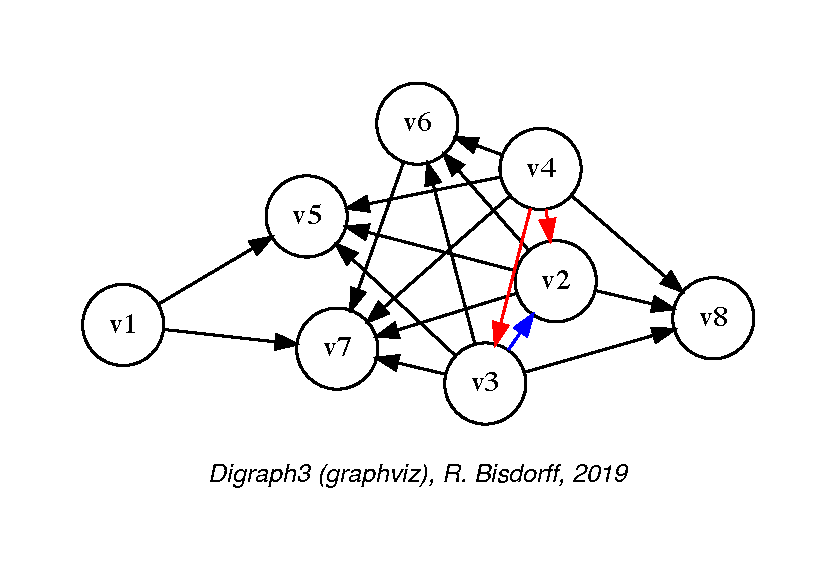
\includegraphics[width=7cm]{Figures/23-10-transOrientDualGraph.pdf}
\caption{Transitive neighbourhoods of the dual graph \texttt{-g}. It is worthwhile noticing that the orientation of \texttt{g} is achieved with a single neighbourhood decomposition, covering all the vertices. Whereas, the orientation of the dual graph \texttt{-g} here needs a decomposition into three subsequent neighbourhoods marked in black, red and blue} 
\label{fig:23.10}       % Give a unique label
\end{figure}
 
Let us recheck these facts by explicitly constructing transitively oriented digraph instances with the \texttt{computeTransitivelyOrientedDigraph()} method\index{computeTransitivelyOrientedDigraph@\texttt{computeTransitivelyOrientedDigraph()}}.
\begin{lstlisting}
>>> og = g.computeTransitivelyOrientedDigraph(\
...                      PartiallyDetermined = True)
>>> print('Transitivity degree: %.3f' %\
...                      (og.transitivityDegree)) 
  Transitivity degree: 1.000
>>> ogd = (-g).computeTransitivelyOrientedDigraph(\
...                      PartiallyDetermined = True)
>>> print('Transitivity degree: %.3f' %\
...                      (ogd.transitivityDegree)) 
  Transitivity degree: 1.000
\end{lstlisting}
The \texttt{PartiallyDetermined = True} flag (see Lines 2 and 7 above) is required here in order to orient only the actual edges of the graphs. Relations between vertices not linked by an edge are put to the indeterminate characteristic value $0$. This allows us to compute, later on, convenient disjunctive digraph fusions.

As both graphs are indeed transitively orientable (see Lines 5 and 10 above), we may conclude that the given random graph \texttt{g} is actually a permutation graph instance. Yet, we still need to find now its corresponding permutation. We therefore implement a recipee given by Martin Golumbic \citep[p. 159]{GOL-2004}.

We will first \emph{fuse} both $og$ and $ogd$ orientations above with an \emph{epistemic disjunction} operated with the symmetric \texttt{o-max} operator (see Section~\vref{sec:2.5}).
\begin{lstlisting}
>>> from digraphs import FusionDigraph
>>> f1 = FusionDigraph(og,ogd,operator='o-max')
>>> s1 = f1.computeCopelandRanking()
>>> print(s1)
  ['v5','v7','v1','v6','v8','v4','v3','v2']
\end{lstlisting}
With the \texttt{computeCopelandRanking()} method\index{computeCopelandRanking@\texttt{computeCopelandRanking()}}, we obtain the linear ordering [\texttt{v5}, \texttt{v7}, \texttt{v1}, \texttt{v6}, \texttt{v8}, \texttt{v4}, \texttt{v3}, \texttt{v2} of the vertices (see Line 5 above).

We reverse now the orientation of the edges in \texttt{og} (see \texttt{-og} in Line 1 below) in order to generate, again by disjunctive fusion, the \emph{inversions} that are produced by the permutation we are looking for.

Computing again a ranking with the \Copeland rule, reveals the permuted list of vertices we are looking for (see Line 4 below).
\begin{lstlisting}
>>> f2 = FusionDigraph((-og),ogd,operator='o-max')
>>> s2 = f2.computeCopelandRanking()
>>> print(s2)
  ['v8','v7','v6','v5','v4','v3','v2','v1']
\end{lstlisting}
Vertex \texttt{v8} is put from position 5 to position 1, vertex \texttt{v7} is put from position 2 to position 2, vertex \texttt{v6} from position 4 to position 3, vertex \texttt{v5} from position 1 to position 4, etc ... . We generate these position swaps for all vertices and obtain thus the required permutation (see Line 5 below).
\begin{lstlisting}
>>> permutation = [0 for j in range(g.order)]
>>> for j in range(g.order):
...     permutation[s2.index(s1[j])] = j+1
>>> print(permutation)
  [5, 2, 4, 1, 6, 7, 8, 3]
\end{lstlisting}

It is worthwhile noticing by the way that transitive orientations of a given graph and its dual are usually \emph{not unique} and, so may also be the resulting permutations. However, they all correspond to isomorphic graphs (see \citep{GOL-2004}). In our case here, we observe two different permutations and their reverses::
\begin{lstlisting}
s1: ['v1', 'v4', 'v3', 'v2', 'v5', 'v6', 'v7', 'v8']
s2: ['v4', 'v3', 'v2', 'v8', 'v6', 'v1', 'v7', 'v5']
(s1 -> s2): [2, 3, 4, 8, 6, 1, 7, 5]
(s2 -> s1): [6, 1, 2, 3, 8, 5, 7, 4]
\end{lstlisting}
And
\begin{lstlisting}  
s3: ['v5', 'v7', 'v1', 'v6', 'v8', 'v4', 'v3', 'v2']
s4: ['v8', 'v7', 'v6', 'v5', 'v4', 'v3', 'v2', 'v1']
(s3 -> s4): [5, 2, 4, 1, 6, 7, 8, 3]
(s4 -> s3) = [4, 2, 8, 3, 1, 5, 6, 7]
\end{lstlisting}
The \texttt{computePermutation()} method\index{computePermutation@\texttt{computePermutation()}} does directly operate all these steps: - computing transitive orientations, - ranking their epistemic fusion and, - delivering a corresponding permutation.
\begin{lstlisting}  
>>> g.computePermutation(Comments=True)
  ['v1', 'v2', 'v3', 'v4', 'v5', 'v6', 'v7', 'v8']
  ['v2', 'v3', 'v4', 'v8', 'v6', 'v1', 'v7', 'v5']
  [2, 3, 4, 8, 6, 1, 7, 5]
\end{lstlisting}

We may finally check that, for instance, the two permutations [2, 3, 4, 8, 6, 1, 7, 5] and [4, 2, 8, 3, 1, 5, 6, 7] observed above, will generate corresponding \emph{isomorphic} permutation graphs.
\begin{lstlisting}  
>>> gtesta = PermutationGraph(\
...             permutation=[2, 3, 4, 8, 6, 1, 7, 5])
>>> gtestb = PermutationGraph(\
  ...           permutation=[4, 2, 8, 3, 1, 5, 6, 7])
>>> gtesta.exportGraphViz('gtesta')
>>> gtestb.exportGraphViz('gtestb')
\end{lstlisting}
\begin{figure}[h]
  % \sidecaption
  [2, 3, 4, 8, 6, 1, 7, 5]\hfill [4, 2, 8, 3, 1, 5, 6, 7]\\
  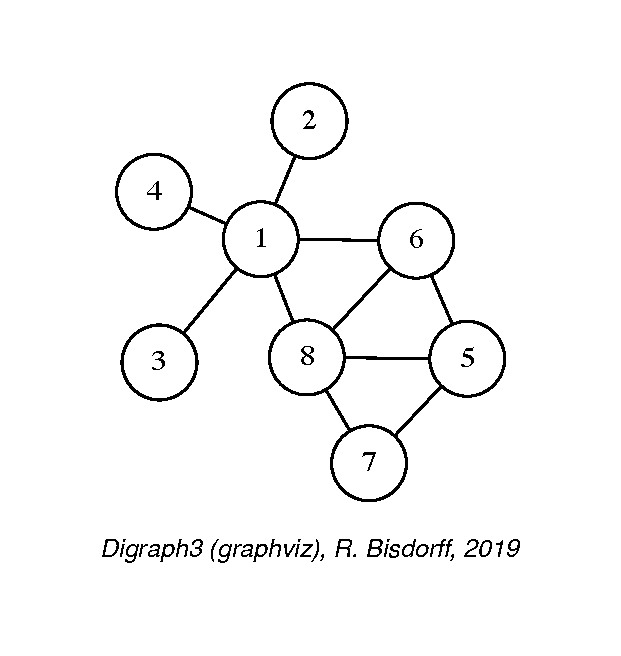
\includegraphics[width=6cm]{Figures/23-11-gtesta.pdf}\hfill
  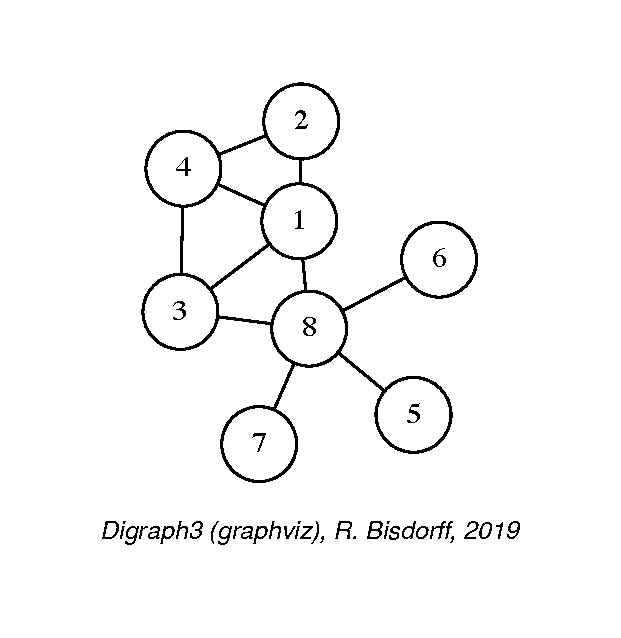
\includegraphics[width=6cm]{Figures/23-11-gtestb.pdf}
\caption{Isomorphic permutation graphs.} 
\label{fig:23.11}       % Give a unique label
\end{figure}
And, we indeed recover in Fig.~\vref{fig:23.11} indeed two isomorphic copies of the original random graph (compare with Fig.~\vref{fig:23.8}).
 
%%%%%%% The chapter bibliography
%\normallatexbib
\clearpage
%\phantomsection
%\addcontentsline{toc}{section}{Chapter Bibliography}
\bibliographystyle{spbasic}
%\typeout{}
\bibliography{03-backMatters/reference}
%\input{02-mainMatters/25-chapterPerfectGraph3.bbl}